\documentclass[a4paper, 10pt]{article}
\usepackage[unicode=true, colorlinks=true, linkcolor=blue, urlcolor=blue]{hyperref}
\usepackage[T2A]{fontenc}
\usepackage[utf8]{inputenc}
\usepackage[russian]{babel}
%\usepackage{indentfirst}
\usepackage{amssymb}
\usepackage{enumitem}
\usepackage{hyperref}
\usepackage{geometry}
\usepackage{mathtools}
\usepackage{setspace}
\usepackage{tikz}
\usepackage{textcomp}
\usepackage{ stmaryrd }
\usepackage{ulem}
\usepackage{ dsfont }
\usepackage{tikzsymbols}
\usepackage{graphicx}
\usepackage{graphicx}
\graphicspath{{img/}}
\DeclareGraphicsExtensions{.pdf,.png,.jpg}


\geometry{a4paper,top=2cm,bottom=2cm,left=2cm,right=2cm}
\usepackage{HWspecial}

%$$\includegraphics{}$$

\title{Коллоквиум 1 по дискретной математике}
\author{Элбакян Сурен  \href{https://t.me/E7SSSS}{@E7SSSS}, \\ Артём Парфенов \href{https://t.me/dunno_0}{@dunno}}
\date{November 2021}
\begin{document}

\maketitle

\tableofcontents

\newpage

\section{Список определений и теорем из курса}

\subsection{Логические значения и логические связки. Задание таблицами истинности.}

%$$\includegraphics{лог.связки.png}$$

Будем рассматривать высказывания, которые обязательно либо \textit{истинны}, либо \textit{ложны}. Из высказываний можно составлять новые, используя \textit{логические связки}.

Значения составных высказываний определяются в зависимости от связки по таблицам истинности. Приведём таблицы истинности самых употребительных связок: конъюнкция $\wedge$ «А и Б», дизъюнкция $\vee$ «А или Б», импликация(логическое следование): «если А, то Б», «Из А следует Б» и равносильности $\equiv$ «А равносильно Б».

\begin{center}
	\begin{table}[h]
		\centering
		\begin{tabular}{|l|l|l|l|l|l|}
			\hline
			\multicolumn{1}{|c|}{A} & B & $A \vee B$ & $A \wedge B$ & $A \to B$ & $A \equiv B $\\ \hline
			0                       & 0 & 0                       & 0                         & 1                      & 1                         \\ \hline
			0                       & 1 & 1                       & 0                         & 1                      & 0                         \\ \hline
			1                       & 0 & 1                       & 0                         & 0                      & 0                         \\ \hline
			1                       & 1 & 1                       & 1                         & 1                      & 1                         \\ \hline
		\end{tabular}
	\end{table}
\end{center}



В импликации $A \to B$ высказывание A - посылка импликации, B - заключение.


\subsection{Законы де Моргана}

Важным примером тавтологий являются законы де Моргана. Они позволяют строить высказывания, равносильные отрицанию конъюнкции или дизъюнкции: \\
$$\neg(A \wedge B) \equiv \neg A \vee \neg B$$  $$\neg(A \vee B) \equiv \neg A \wedge \neg B$$

\textbf{Доказательство тождеств:}

Отрицание конъюкции ложно тогда и только тогда, когда конъюкция истинна, то есть $A = B = 1$. Дизъюнкция ложна тогда и только тогда, когда каждый её член ложен, то есть $\neg A = \neg B = 0$. Эти условия равносильны.

Отрицание дизъюнкции истинно тогда и только тогда, когда дизъюнкция ложна, то есть $A = B = 0$. Конъюкция  истинна тогда и только тогда, когда каждый её член истинен, то есть $\neg A = \neg B = 1$.Эти условия равносильны

\subsection{Доказательства разбором случаев. Примеры.}

Проверка логического тождества по таблицам истинности — это частный случай широко применяемого и хорошо известного приёма доказательств: разбора случаев. Для доказательства A мы строим равносильное высказывание, которое состоит из конъюнкции нескольких высказываний и доказываем по очереди каждый член конъюнкции. Тут важно не пропустить какой-нибудь случай, то есть доказать равносильность A и конъюнкции. В случае проверки по таблицам всё довольно просто: нужно не забыть проверить каждую строчку.

Однако для доказательства логических тождеств необязательно проверять каждую строчку таблицы истинности составного высказывания. Зачастую достаточен неполный разбор случаев.

\textbf{В качестве примера} докажем логические тождества дистрибутивности конъюнкции и дизъюнкции (тут даже лучше, чем с числами — есть две тавтологии):

$$A \wedge (B \vee C) \equiv (A \wedge B) \vee (A \wedge C)$$

$$A \vee (B \wedge C) \equiv (A \vee B) \wedge (A \vee C)$$

Будем использовать очевидные тавтологии упрощения: $X \vee 0 = X$, $X \vee 1 = 1$, $X \wedge 0 = 0$, $X \wedge 1 = X$

Доказательство дистрибутивности конъюкции и дизъюнкции. Разберём два случая: $A = 1$ и $A = 0$.

Если $A = 0$, то левая часть первого тождества равна $0$, а правая $0 \vee 0 = 0$. Обе части второго высказывания обращаются в $B \wedge C$, поэтому они равны.

Если $A = 1$, то разбор аналогичный: обе части первого тождества обращаются в $B \vee C$; левая часть второго тождества равна 1, а правая $1 \wedge 1 = 1$


\subsection{Доказательство от противного. Примеры.}


Допустим, мы хотим доказать утверждение А. Для этого мы выводим из его отрицания $\neg A$ противоречие, то есть докажем, что некоторое высказывание $B$ одновременно истинно и ложно(более формально, докажем $B$ и $\neg B$). Другими словами, докажем истинность составного высказывания $\neg A \rightarrow (B \wedge \neg B)$. Заключение этой импликации ложно. Поскольку сама импликации истинна, то и её посылка ложна. То есть, $A$ истинно, что и требовалось доказать.

\textbf{Примеры}. За пример сойдёт доказательство иррациональности числа $\sqrt{2}$. Также можно какое-нибудь док-во из домашек(задачки в главе 2)

\subsection{Принцип контрапозиции. Примеры}

Ещё один важный приём доказательства основан на тавтологии, которая называется принципом контрапозиции:

$$A \rightarrow B \equiv \neg B \rightarrow \neg A$$

Доказательство: Используем для обеих частей представление импликации через дизъюнкцию. Получаем равносильное тождество

$$\neg A \vee B \equiv \neg \neg B \vee \neg A$$

Заметим, что $\neg \neg B \equiv B$ и дизъюнкция коммутативна, поэтому тождество - тавтология.

\textbf{Пример.} Докажем такое утверждение: если число $x$ - иррациональное, то $\sqrt{x}$ - тоже иррациональное.

Закон контрапозиции говорит, что если $\sqrt{x}$ рациональное, то и $x$ рациональное. А это уже легко доказать:квадрат обыкновенной дроби является обыкновенной дробью


\subsection{Свойства дизъюнкции и конъюнкции(ассоциативность, дистрибутивность, коммутативность).}


$A \wedge B \equiv B \wedge A$, \qquad $A \vee B \equiv B \vee A$ - \textbf{коммутативность} \\

\noindent $A \wedge (B \wedge C) \equiv (A \wedge B) \wedge C$, \qquad $A \vee (B \vee C) \equiv (A \vee B) \vee C$ - \textbf{ассоциативность} \\

\noindent $A \wedge (B \vee C) \equiv (A \wedge B) \vee (A \wedge C)$, \qquad $A \vee (B \wedge C) \equiv (A \vee B) \wedge (A \vee C)$ - \textbf{дистрибутивность}


\subsection{Множества, теоретико-множественные операции. Взаимосвязь множеств и булевой логики}

Множество — это совокупность каких-то элементов. Природа элементов и взаимоотношения между ними не важны. Существенно лишь, какие элементы в входят в множество, а какие — нет. Поэтому множество полностью определяется своими элементами. Два множества A и B называются равными, если каждый элемент множества A является элементом множества B, а каждый элемент множества B является элементом множества A.

Множество A является подмножеством множества B, если каждый элемент множества A принадлежит множеству B (обозначение $A \subseteq B$). Высказывание «элемент x принадлежит множеству A» (обозначение $x \in A$) истинно, если в A есть элемент x, и ложно в противном случае.
\\

\textbf{Объединение множеств}. Обозначение $A \cup B$. Это множество состоящие в точности из тех элементов, которые принадлежат хотя бы одному из множеств A и B. В формальной записи это определение выглядит так:
$$A \cup B = \{x \colon (x \in A) \vee (x \in B)\}$$ \\

\textbf{Пересечение множеств}. Обозначение $A \cap B$. Это множество состоящие в точности из тех элементов, которые принадлежат обоим множествам. В формальной записи это определение выглядит так:
$$A \cap B = \{x \colon (x \in A) \wedge (x \in B)\}$$ \\

\textbf{Разность множеств}. Обозначение $A \setminus B$. Это множество состоящие в точности из тех элементов, которые принадлежат множеству A, но не принадлежат множеству B. В формальной записи это определение выглядит так:
$$A \setminus B = \{x \colon (x \in A) \wedge \neg (x \in B)\}$$ \\

\textbf{Симметрическая разница множеств}. Обозначение $A \triangle B$. Это множество состоящие в точности из тех элементов, которые принадлежат ровно одному из множеств, либо A, либо B. В формальной записи это определение выглядит так:
$$A \triangle B = \{x \colon ((x \in A) \wedge \neg (x \in B)) \vee (\neg (x \in A) \wedge (x \in B))\}$$ \\


\textbf{Импликация} отвечает за $A \subseteq B$(Если $x \in A$, то $x \in B$)\\

\textbf{Равносильность} отвечает за равенство множеств



\subsection{Принцип математической индукции. Принцип полной математической индукции}

\textbf{Принцип математической индукции}. Пусть для последовательности утверждений

$$A_1, A_2, ..., A_n, ...$$ занумерованных целыми положительными числами верны утверждения:

\textbf{База индукции} $A_1$ - истинно.

\textbf{Шаг индукции:} $A_n \to A_{n + 1}$ истинно для любого n. Посылку импликации $A_n$ называют индуктивным предположением.

Тогда $A_n$ истинно для любого n.


\textbf{Принцип полной математической индукции}. Пусть для последовательности утверждений

$$A_1, A_2, ..., A_n, ...$$ занумерованных целыми положительными числами истинно утверждения: «для любого n из истинности $A_i$ при всех $i < n$ следует истинность $A_n$». Тогда $A_n$ истинно для любого n.


\subsection{Принцип кроликов(он же «принцип Дирихле»)}

\textbf{Принцип кроликов.} Если $k > n$ и $k$ кроликов посадили в $n$ клеток, то хотя бы в одной клетке сидит хотя бы два кролика.

\subsection{Числа Фибоначчи, формула для чисел Фибоначчи.}


Рассмотрим \textit{последовательность} Фибоначчи:

$$1, 1, 2, 3, 5, 8, 13, 21, 34, \dots, $$

в которой первые два числа равны единице, а каждое следующее равно сумме двух предыдущих. Обычный способ задания таких рекуррентных последовательностей выглядит так: $F_0 = 1; F_1 = 1; F_{n + 1} + F_n, \  \forall n \geqslant 0$

$$F_n = \frac{\psi^{n + 1} - \varphi^{n + 1}}{\sqrt{5}}, \ \text{где} \ \psi = \frac{1 + \sqrt{5}}{2}, \ \varphi = \frac{1 - \sqrt{5}}{2}$$



\subsection{Ориентированные и неориетированные графы. Степени вершин.}

\textbf{Простой неориентированный граф} — это множество вершин V и множество рёбер E. Рёбрами являются 2-элементные подмножества множества V.


\textbf{Теорема}. Сумма степеней всех вершин графа равна удвоенному числу его рёбер

\textbf{Простой ориентированный граф
(орграф)} — это конечное множество вершин V и множество рёбер E. Рёбрами являются упорядоченные пары вершин (то есть последовательности длины 2).

В неориентированных графах степень вершины равна количеству инцидентных ей рёбер. В орграфах часть рёбер входит в вершину, часть — выходит. Их считают по отдельности. Исходящая степень вершин равна числу рёбер, выходящих из этой вершины. Входящая степень равна числу рёбер, входящих в вершину. Если в вершине v
есть петля $e = (v, v)$, то вершина v является и началом и концом петли e. Поэтому петля даёт вклад 1 и в исходящую степень, и во входящую.

\textbf{Лемма}. Сумма исходящих степеней всех вершин графа равна сумме входящих степеней всех вершин: обе суммы равна числу рёбер графа.



\subsection{Задание графов матрицами смежности и инцидентности.}

Матрица смежности графа: на пересечении i-й строки и j-го столбца стоит 1, если вершины i, j соседние; иначе там стоит 0.


Таким образом, матрица смежности графа с n вершинами — это таблица с n строками и n столбцами (как говорят, квадратная матрица порядка n).


Матрица инцидентности графа: на пересечении i-й строки и j-го столбца стоит 1, если вершина i инцидентна ребру j; иначе там стоит 0


Таким образом, матрица инцидентности - это матрица размера $n \times m$, где n - кол-во строк(вершин графа), m - кол-во столбцов(рёбер графа)


\subsection{Примеры графов:полный граф, булев куб, граф-путь, граф-цикл.}


$$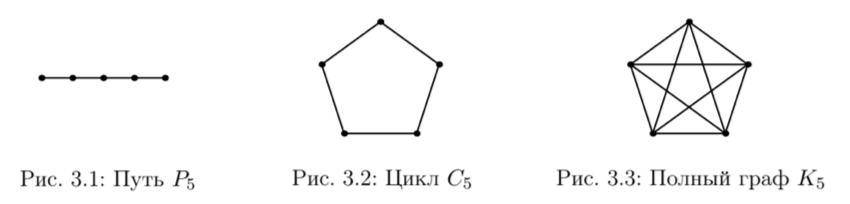
\includegraphics{graphs_ex.png}$$


$$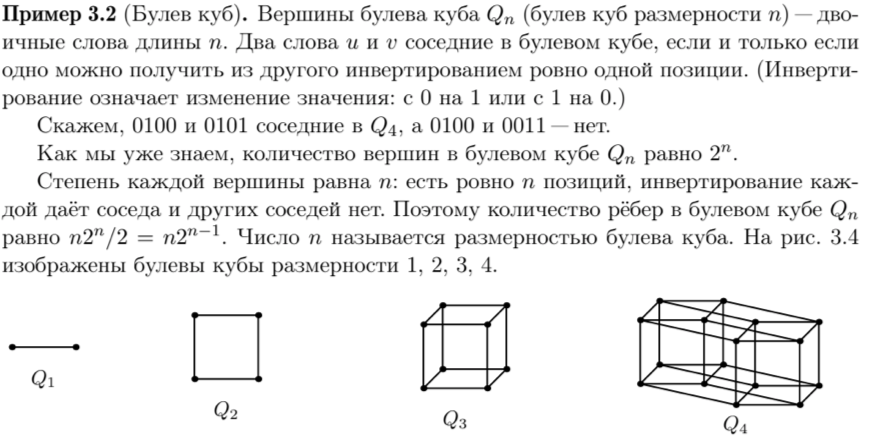
\includegraphics{binary_cube.png}$$


\subsection{Циклы и пути в графах}

\textbf{Цикл} - замкнутый путь по графу, то есть такой путь, у которого начало совпадает с концом.

\textbf{Простой цикл} - цикл, в котором все вершины различны(за исключением начала и конца)

\textbf{Путь} по графу - последовательность вершин $u_1, u_2, ..., u_t$, в которой стоящие рядом члены($u_{i}, u_{i+1}$ при все допустимых i) соединены ребром

\textbf{Простой путь} -  путь, в котором все вершины различны


\subsection{Отношение достижимости и компоненты связности графа. Связные графы.}



\textbf{Рефлексивность}. $u_1 \in C(u_1)$ (вершина достижима из самой себя).

\textbf{Симметричность}. $u_1 \in C(u_2)$ равносильно $u_2 \in C(u_1)$.

\textbf{Транзитивность}. Если $u_2 \in C(u_1)$ и $u_3 \in C(u_2)$, то $u_3 \in C(u_1)$.  \\

\textbf{Лемма.} Если $w \in C(v_1) \cap C(v_2)$, то $C(v_1) = C(v_2)$. Области достижимости не пересекаются или совпадают.


Лемма говорит, что области достижимости не пересекаются или совпадают. Таким образом, мы получаем разбиение множества вершин графа на подмножества. Каждое такое подмножество может быть представлено как область достижимости любого элемента из этого множества.

Удобно не упоминать этот случайно выбранный элемент. Поэтому используется такая терминология. Компонента связности графа—это область достижимости некоторой вершины этого графа.

\textbf{Компоненты связности} — это в точности максимальные по включению множества вершин, индуцирующие связный граф.

Граф связный, если у него одна компонента связности.


\subsection{Деревья и леса. Мосты. Критерии деревьев.}

\textbf{Дерево} - такой связный граф, что выбрасывание любого ребра даёт несвязный граф.

\textbf{Мост} - такое ребро в графе, что его удаление увеличивает количество компонент связности

\textbf{Критерии дерева}.Равносильны следующие свойства простых неориентированных графов:

(1) каждое ребро - мост.

(2) для любых связанных вершин $u, v$ существует единственный простой путь из $u, v$

(3) нет простых циклов длины больше 2.

\textbf{Теорема}. Графы, у которых размерность равна 0, - это в точности леса, то есть графы, у которых каждое ребро - мост ($dim(G) = m - n + c$, m-ребра, n-вершины, c-компоненты связности)

\textbf{Следствие.} Связный граф является деревом тогда и только тогда, когда число рёбер в нём на единицу меньше числа вершин.


\subsection{Компоненты сильной связности в ориентированных графах.}

Будем говорить, что вершина $u$ сильна связана с вершиной $v$, если $u$ достижима из $v$ и наоборот.

Через $C(u)$ обозначим множество вершин $v$, которые сильно связаны с $u$. Эти множества обладают теми же свойствами, что и компоненты связности обычного ориентированного графа и называются компонентами сильной связности.

\textbf{Лемма.} Для любого графа и любых его вершин $u_1, u_2, u_3$ выполняются следующие свойства:

1. $u_1 \in C(u_1)$ (вершина сильно связана сама с собой)

2. $u_1 \in C(u_2)$ равносильно $u_2 \in C(u_1)$

3. Если $u_2 \in C(u_1)$ и $u_3 \in C(u_2)$, то $u_3 \in C(u_1)$


\textbf{Лемма.} Если $w \in C(u_1) \cap C(u_2)$, то $C(u_1) = C(u_2)$. Компоненты сильной связности не пересекаются или совпадают.

Если всё множество вершин орграфа образует компоненту сильной связности, такой орграф называется сильно связным. Примером сильно связного графа является ориентированный цикл



\subsection{Ациклические графы}

Орграф называется ациклическим, если в нём нет циклов длины больше 0. Другими словами, никакие две различные вершины не являются сильно связанными. Название объясняется следующей теоремой. В ней мы требуем отсутствия петель в орграфе\\

\textbf{Теорема}. Следующие свойства орграфа без петель равносильны:

1. Каждая компонента сильной связности состоит из 1 вершины

2. Ограф ациклический

3.Вершины орграфа можно пронумеровать натуральными числами таким образом, чтобы все рёбра вели из вершины c меньшим номером в вершину с большим.\\

\textbf{Лемма}. В ациклическом оргафе есть вершина, из которой не выходит ни одного ребра, и есть вершина, в которую не входит ни одно ребро


\subsection{Эйлеровы графы}
Цикл (в неориентированном или ориентированном графе) называется эйлеровым, если он проходит по всем рёбрам графа ровно по одному разу (любое ребро соединяет соседние вершины в цикле, и никакое ребро не делает это дважды).

Граф называется эйлеровым, если в нём есть эйлеров цикл.

Есть простой критерий эйлеровости графов и орграфов. Прежде всего заметим, что добавление и удаление изолированных вершин, то есть тех вершин, из которых
не выходит и в которые не входит ни одного ребра, не изменяет свойство эйлеровости графа.

\textbf{Теорема 1.} В ориентированном графе без изолированных вершин существует эйлеров цикл тогда и только тогда, когда граф сильно связен и у любой вершины входящая степень равна исходящей

\textbf{Теорема 2.} Неориентированный граф без вершин нулевой степени содержит эйлеров цикл тогда и только тогда, когда он связен и степени всех вершин чётны.


\subsection{k-раскрашиваемые графы. Критерий 2-раскрашиваемости}

Правильной раскраской вершин неориентированного графа $G(V, E)$ в k цветов называется такое присваивание вершинам графа чисел (цветов) от 1 до k, что присвоенные смежным вершинам числа различны. Если для графа существует хотя бы одна правильная раскраска в k цветов, граф называется k-раскрашиваемым

\textbf{Теорема.} 2-раскрашиваемые графы это в точности графы, в которых длины всех циклов чётные.


\subsection{Паросочетания.}

Паросочетанием называется граф, у которого степени всех вершин не больше 1. Когда говорят о паросочетании в графе, имеют в виду (рёберный) подграф этого графа: множество вершин и часть рёбер между ними, которые образуют паросочетание.

$$\includegraphics{matсhing.png}$$

Такой граф устанавливает взаимно однозначное соответствие между частью вершин левой доли и частью вершин правой доли. В частности, если паросочетание совершенное(нет изолированных вершин, то есть вершин степени 0), то рёбра паросочетания устанавливают взаимно однозначное соответствие между вершинами левой и правой долей. Такое возможно, если размеры долей одинаковы




\subsection{Двудольные графы.}

Двудольным графом называется неориентированный граф, в котором вершины заранее разделены на две доли — левую и правую, и все рёбра соединяют вершины из разных долей (нет рёбер, соединяющих вершины одной доли). Другими словами, чтобы задать двудольный граф, надо указать два конечных множества L (левую долю) и R (правую долю) и указать, какие вершины левой доли соединены с какими вершинами правой доли

Из определения бинарного отношения сразу следует, что двудольные графы графы с долями $L, R$ по сути то же самое, что бинарные отношения на множествах $L, R$ (то есть тоже самое, что подмножества декартова произведения $L \times R$



\subsection{Теорема Холла}

\textbf{Теорема Холла.} Если для каждого множества $X$ вершин двудольного графа $G = (L \cup R, E)$ множество соседей $G(X) \subseteq R$ содержит не меньше вершин, чем $X$, то в графе $G$ есть паросочетания размера $|L|$


\subsection{Вершинные покрытия.Теорема Кёнига.}


\textbf{Вершинным покрытием} называется такое множество вершин S, что для любого ребра хотя бы один из концов лежит в S. Нетрудно проверить, что дополнение к вершинному покрытию — независимое множество и, наоборот, дополнение к независимому множеству — вершинное покрытие. Для двудольных графов вершинные покрытия оказываются связанными с паросочетаниями.


\textbf{Теорема Кёнига}.В любом двудольном графе максимальный размер паросочетания равен минимальному размеру вершинного покрытия


\subsection{Клики и независимые множества. Теорма Рамсея}


\textbf{Независимое множество} вершин в графе - множество вершин, в котором никакая пара вершин не соединена ребром


\textbf{Кликой} называется множество вершин графа, каждая пара которых соединена ребром


\textbf{Теорема Рамсея}. Для любых $k, n$ найдётся такое число $N_0$, что в любом графе на $N \geqslant N_0$ вершинах есть или клика размера k, или независимое множество размера $n$.


\subsection{Функции. Образы и прообразы множеств}

\textbf{Графиком функции Г$_f$} из множества A в множество B называется такое подмножество Г$_f \subseteq A \times B$ декартовка произведения, что для каждого $a \in A$ есть не более одной пары $(a, b) \in$ Г$_f$

Пусть $X \subseteq A$ - подмножество множества A. Функция $f$ сопоставляет ему \textbf{образ} $f(X) \subseteq B$ подмножества X. По определению $f(x)$ состоит в точности из тех элементов множества B, которые являются значениями элементов из X.

Функция $f$ устанавливает также однозначное соответствие и в обратную сторону — между подмножествами множества $B$ и подмножествами множества $A$. Подмножеству $Y \subseteq B$ можно сопоставить полный прообраз $f^{-1}(Y) \subseteq A$ подмножества $Y$ . По определению $f^{-1}(Y)$ состоит в точности из тех элементов $A$, значения которых лежат в $Y$.


\subsection{Виды функций: инъекция, биекция и сюръекция}

%$$\includegraphics{функции.png}$$

Тотальная функция $f \colon A \to B$ называется \textit{инъекцией}, если значения функции в различных точках различны. Более формально: f - инъекция, если $x_1 \neq x_2$ влечёт $f(x_1) \neq f(x_2)$. (Часто удобна контрапозиция этого утверждения)

$$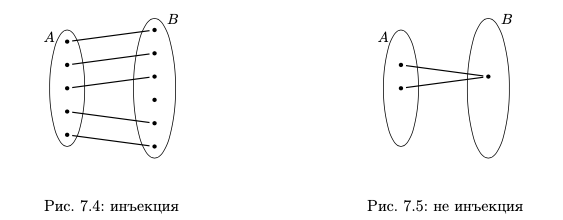
\includegraphics[scale=0.6]{inj.png}$$

Тотальная функция $f \colon A \to B$ называется \textit{сюръекцией}, если область значений совпадает со всем множеством B, то есть если $\forall y \in B \ \exists x \in A \colon f(x) = y$

Пример сюръекции изображён на рис 7.6. Примеры не сюръекций изображены на рисунке 7.7: для сюръективной функции не должно быть точек справа, в которые не ведёт ни одного ребра.

$$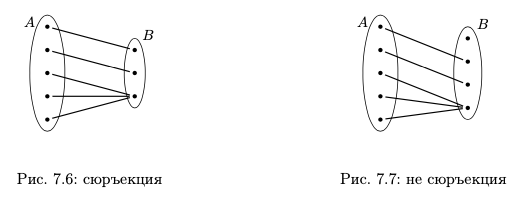
\includegraphics[scale=1.22]{surj.png}$$


Наконец, тотальная функция $f \colon A \to B$ называется биекцией, если она одновременно является и инъекцией, и сюръекцией. Другими словами, функция является биекцией, если всякому элементу из A соответствует ровно один элемент из B.

Поэтому биекцию ещё называют \textit{взаимно однозначным соответствием} между множествами.



\subsection{Свойство инъекций, сюръекций и биекций на конечных множествах}

\textbf{Лемма}. Для тотальных функций из конечного множества в конечное выполняются такие свойства:

1. если $f\colon A \to B$ сюръекция, то $|A| \geqslant |B|$

2. если $f\colon A \to B$ инъекция, то $|A| \leqslant |B|$

3. если $f\colon A \to B$ биекция, то $|A| = |B|$


\subsection{Композиция функций. Ассоциативность композиции}

Для функции $f$ из множества $A$ в множество $B$ и функции $g$ из множества $B$ в множество $C$ композицией $g \circ f$ этих функций является такая функция из $A$ в $C$, которая определена на тех $x$ из области определения функции $f$, для которых $f(x)$ принадлежит области определения функции $g$, и равна $g(f(x))$. Это функция, так как каждому значению аргумента $x \in A$ сопоставляется не более одного элемента из $C$.

Композиция функций обладает свойством ассоциативности:

$$(f \circ g) \circ h = f \circ (g \circ h)$$

$$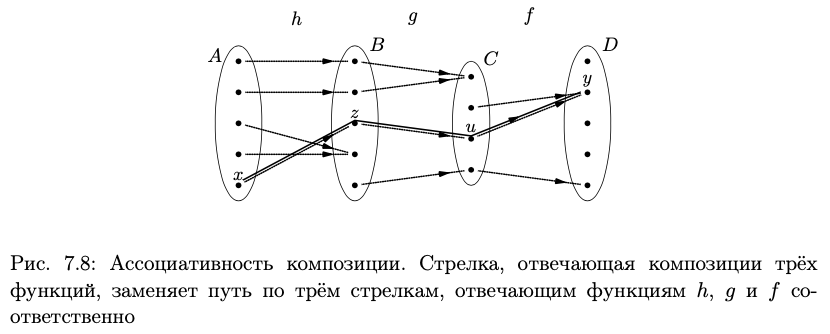
\includegraphics{composition.png}$$


\subsection{Обратная функция. Алгебраическая характеризация}

Для биекции $f\colon A \to B$ (взаимно однозначного отображения) определена обратная функция (или обратное отображение) $f^{-1}$: если f отображает $x$ в $y$, то обратная функция $f^{-1}$ отображает $y$ в $x$. Инъективность $f$ гарантирует, что это действительно функция, а сюръективность $f$ гарантирует, что эта функция определена на всём $B$.

\textbf{Теорема}. Если для отображение $f: A \to B$ и $g\colon B \to A$ выполнены два равенства $g \circ f = id_A$ и $f \circ g = id_B$, то функция $f$ является биекцией и $g$ обратна к $f$.



\subsection{Равномощные множества. Свойства мощности}

Множества равномощны, если существует биекция $f\colon A \to B$ \\

\textbf{Лемма. Рефлексивность}: каждое множеству равномощно самому себе. \\

\textbf{Симметричность}. Если A равномощно B, то и B равномощно A для любых множеств A, B. \\

\textbf{Транзитивность}. Если A равномощно B и B равномощно C, то A равномощно C.


\subsection{Счетные мощности}

\textbf{Определение}. Множество называется счетным, если оно равномощно множеству натуральных чисел $\mathbb{N} = \{1, 2, 3, ...\}$

Само множество $\mathbb{N}$, очевидно, счётно (рефлексивность равномощности).


\subsection{Множества мощности континуум}



\textbf{Определение}. Множество имеет мощность континуум, если оно равномощно множеству бесконечных двоичных последовательностей $\{0, 1\}^{\mathbb{N}}$

\textbf{Теорема}. Отрезок $[0, 1]$ имеет мощность континуум(интервал $(0, 1)$ также имеет мощность континуум).

\textbf{Следствие}. Мощность действительных чисел $\mathbb{R}$ имеет мощность континуум.


\subsection{Бинарные отношения}

\textbf{Определение.} Бинарным отношением на множествах $A$ и $B$ называется любое подмножество $R$ декартова произведения $A \times B$. Если $(x, y) \in R$ говорят, что $x$ и $y$ находятся в отношении $R$ (порядок важен).

График функции—это пример бинарного отношения с дополнительным свойством: каждый элемент a находится в отношении не более, чем с одним элементом B.

Двудольный граф на долях L и R задаёт бинарное отношение на множествах A и B: вершины находятся в отношении, если они связаны ребром. В случае $A = B$
получаем определение ориентированного графа.

Рассмотрим множество пар действительных чисел $(x, y)$, для которых $x < y$. Это множество по определению задаёт бинарное отношение «строго меньше» на действительных числах.

\subsection{Композиция бинарных отношений. Ассоциативность композиции.}

\textbf{Определение} Пусть даны два отношения $R \subset A \times B$ и $S \subset B \times C$. Их \textit{композицией} называется отношение $S \circ R \subseteq A \times C$, определяемое так:

$$(x, z) \in S \circ R \Longleftrightarrow \exists \ y \in B \colon (x, y) \in R \ \wedge \ (y, z) \in S$$

Обратите внимание, что (1) композиция определена не для всех отношений, необходимо совпадение второго множества в первом отношении и первого во втором; (2) порядок записи отношений в композиции важен, если R и S - функции, то композиция их графиков как бинарных отношений в точности совпадает с графиком композиции функций.

Если задавать отношения на конечных множествах матрицами, композиция отношений задаётся формулой, напоминающей формулу произведения числовых матриц, но операции в этой формуле логические:

$$\displaystyle (S \circ R)(x, y) = \bigvee_{z \in B}(R(x, z) \wedge S(z, y))$$

Как и умножение числовых матриц, композиция отношения обладает свойством ассоциативности.

\textbf{Лемма.} Если $R \subset A \times B, S \subset B \times C \ \text{и} \ T \subset C \times D \to (R \circ S) \circ T = R \circ (S \circ T)$



\section{Вопросы на знание доказательств}


\subsection{Формула для чисел Фибоначчи}

$F_n = \frac{a^{n + 1} - b^{n + 1}}{\sqrt{5}}$, где $a = \frac{1 + \sqrt{5}}{2}$, $b = \frac{1 - \sqrt{5}}{2}$ \\

Заметим, что для наших $a, b$ верно равенство $a^2 = a + 1$ и $b^2 = b + 1$, так как $a, b$ -  корни уравнения $x^2 - x -  1 = 0$


Докажем методом полной математической индукции. 

База: нетрудно проверить, что при $n = 0$ и $n = 1$ формула верна.


Шаг индукции: покажем, что если верно для всех k от $\{1, ... n + 1 \}$, то верно для $n + 2$ 


$\displaystyle F_{n + 2} = F_{n + 1} + F_n = \frac{a^{n + 2} - b^{n + 2}}{\sqrt{5}} + \frac{a^{n + 1} - b^{n + 1}}{\sqrt{5}} = \frac{1}{\sqrt{5}}(a^{n + 1}(a + 1) - b^{n + 1}(b + 1)) = \frac{a^{n + 3} - b^{n + 3}}{\sqrt{5}}$(последний переход сделали благодаря замечанию выше) $\to$ из принципа полной математической индукции формула верна $\hfill \square$



\subsection{Формула для суммы степеней вершин в графе}

\textbf{Для неориентированного графа}. Построим матрицу инцидентности. Суммируя единицы в одной строке мы получим степень вершины, следовательно, просуммировав единицы по строкам мы получим сумму степеней всех вершин нашего графа. С другой стороны, суммируя единицы по столбцам, мы получим удвоенное количество рёбер, так как в каждом столбце есть две единицы(так как у ребра есть два конца). Зная, что сумма по строка и по столбцам, получаем, что сумма степеней всех вершин графа равна удвоенному количеству рёбер.

\textbf{Для ориентированного графа}. Каждое ребро имеет одно начало (выходит из какой-то вершины) и поэтому учитывается по разу, когда мы складываем исходящие степени всех вершин. Аналогично для концов рёбер.

$\hfill \square$

\subsection{Свойства отношения достижимости в неориентированном графе(рефлексивность, симметричность, транзитивность)}



\textbf{Рефлексивность}. $u_1 \in C(u_1)$ (вершина достижима из самой себя). $u_1$ - путь в любом графе, поэтому $u_1$ связана сама с собой. \\

\textbf{Симметричность}. $u_1 \in C(u_2)$ равносильно $u_2 \in C(u_1)$. Если $u_1, v_1, v_2, ... v_s, u_2$ - путь, то и $u_2, v_s, ... v_2, v_1, u_1$ также путь(те же вершины, но в обратном порядке). Поэтому достижимость $u_2$ из $u_1$ равносильна достижимости $u_1$ из $u_2$. \\

\textbf{Транзитивность}. Если $u_2 \in C(u_1)$ и $u_3 \in C(u_2)$, то $u_3 \in C(u_1)$. Если $u_2, v_1, v_2, ... v_s, u_1$ - путь и $u_2, w_1, ... w_s, u_3$ - путь, то в этом графе также есть путь $u_3, w_s, ... w_1, u_2, v_1, ... v_s, u_1$, то есть путь из $u_3$ в $u_1$


\subsection{Разбиение неориентированного графа на компоненты связности}

\textbf{Лемма.} Если $w \in C(v_1) \cap C(v_2)$, то $C(v_1) = C(v_2)$. Области достижимости не пересекаются или совпадают.

\medskip

\textbf{Доказательство.} Поскольку $w$ достижима из $v_1$ (определение), а $v_2$ достижима из w (свойство симметричности), то $v_2$ достижима из $v_1$ (свойство транзитивности). Значит, и $v_1$ достижима из $v_2$ (свойство симметричности)


Пусть $x \in C(v_1)$. Тогда $x \in C(v_2)$, свидетельством тому путь из $v_2$ в $v_1$, продолженный путём из $v_1$ в $x$. Значит, $C(v_1) \subseteq C(v_2)$.

Верно и обратное: $C(v_2) \subseteq C(v_1)$ (поменяем индексы в рассуждении). Значит, $C(v_1) = C(v_2)$. \\



Лемма говорит, что области достижимости не пересекаются или совпадают. Таким образом, мы получаем разбиение множества вершин графа на подмножества. Каждое такое подмножество может быть представлено как область достижимости любого элемента из этого множества.

Удобно не упоминать этот случайно выбранный элемент. Поэтому используется такая терминология. Компонента связности графа—это область достижимости некоторой вершины этого графа. $\hfill \square$

\medskip

\textbf{Теорема.} \textit{Компоненты связности - это в точности  максимальные по включению множества вершин, индуцирующие связный граф.}

Условие теоремы означает фактически два утверждения:

(1) любое множество, строго содержащее компоненту связности (все вершины компоненты и ещё хотя бы одну) индуцирует несвязный граф.

(2) любое множество, индуцирующее связный граф, содержится в какой-то компоненте связности.

\textbf{Доказательство.}

(1) Если $X \supset C(v)$ (этот знак означает строгое включение), то $\langle X \rangle$ несвязный: из вершины $x \in X \setminus C(v)$ недостижима $v$.

(2) Пусть $X$ - множество, индуцирующее связный граф, $v \in X$. Поскольку $\langle X \rangle$ связный, то $C(v) \supseteq X$ (вершины из X достижимы из v даже если запрещено выходить за пределы X). 

$\hfill \square$


\subsection{Критерии лесов: графы без простых циклов, графы с единственностью простых путей.}

\textbf{Критерии дерева}.Равносильны следующие свойства простых неориентированных графов:

(1) ребро - мост.

(2) для любых связанных вершин $u, v$ существует единственный простой путь из $u, v$

(3) нет простых циклов длины больше 2. \\

\textbf{Графы с единственностью простых путей. Доказательство. $(1) \to (2)$} Равносильно контрапозиции $\neg(2) \to \neg(1)$ Пусть между вершинами $u$ и $v$ есть два разных пути

$$(u = x_0), x_1, ..., x_r, (v = x_{r + 1})$$
$$(u = y_0), y_1, ..., y_s, (v = y_{s + 1})$$

Начинаются эти пути в одной вершине, но полностью совпадать не могут. Возьмём наибольшее общее начало этих путей, то есть максимально возможное i, для которого $x_j = y_j$ для всех $0 \leqslant j \leqslant i$. Тогда $x_{i + 1} \neq y_{i + 1}$ и потому ребро $\{x_i,x_{i+1} \}$ не входит во второй путь. Действительно, в противном случае этот второй путь не простой: вершина $y_i = x_i$ встретится в нём по крайне мере дважды: второй раз случится, когда $\{y_t, y_{t + 1}\}= \{x_i, x_{i + 1}\}$, по построение $t > i$

Докажем, что ребро $\{x_i, x_{i+1}\}$ — не мост. При удалении этого ребра из графа вершины $x_i, x_{i+1}$ остаются в одной компоненте связности: они связаны (необязательно простым) путём.

$$x_i, x_{i-1}, ... , x_1, u, y_1, ..., y_s, v, x_r, x_{r-1}, ... , x_{i+1}$$

Остальные области достижимости (отличные от $C(x_i))$ не изменяются: пути из таких вершин не проходят через ребро $\{x_i,x_{i+1}\}$. $\hfill \square$

\medskip


\textbf{Графы без простых циклов. Доказательство.$(2) \to (3)$}
 Пусть в графе $G$ есть простой цикл $u_0, u_1,...,u_t = u_0, t > 2$.

Вершины $u_0$ и $u_1$ соседние, а значит связанные в этом графе, причём есть по крайней мере два разных простых пути с концами в этих вершинах: $(u_0, u_1)$ (путь из одного ребра) и путь по остальным рёбрам цикла $(u_0 = u_t, u_{t-1}, . . . , u_2, u_1)$ (здесь важно, что длина цикла больше 2). $\hfill \square$

\medskip

\textbf{Доказательство. $(3) \to 1$}. Равносильно контрапозиции $\neg(1) \to \neg(3)$

Пусть ребро $e = \{x, y\}$ можно удалить из графа $G$ и полученный граф $G' = G - e$ остаётся связным. Это значит, что вершины $x, y$ связанные в $G'$ $\to$ в графе $G'$ есть простой путь $x, u_1, u_2, ..., u_t, y$. Все вершины этого пути различные.

Но тогда в графе $G$ есть простой цикл $x, u_1, u_2, u_3, ..., u_t, y, x$ и, так как $x \neq y$, то длина этого цикла 2. \\

Поскольку мы доказали циклическую цепочку импликаций $(2) \to (1) \to (3) \to (2)$, все эти утверждения равносильны (если хотя бы одно истинно, остальные два тоже истинны). $\hfill \square$


\subsection{Критерий для деревьев: связный граф, в котором разность количества вершин и рёбер 1}

\textbf{Критерий}. Связный граф является деревом тогда и только тогда, когда число рёбер в нём на единицу меньше числа вершин.(ниже будет доказательство не из конспекта, поэтому проверьте его прежде, чем поверить) \\

\textbf{Доказательство висячей вершины(пригодится ниже)}.
Рассмотрим произвольную вершину дерева и пойдём по любому выходящему из неё ребру в другую вершину. Если из новой вершины больше рёбер не выходит, то мы остаёмся в ней, а в противном случае идём по любому другому ребру дальше. В этом путешествии мы никогда не сможем попасть в вершину, в которой уже побывали(так как в дереве нет циклов). Так как у графа конечное число вершин, то наше путешествие когда-нибудь закончится. Но закончиться оно может только в висячей вершине(так как из неё пойти дальше не можем, следовательно, связана она только с вершиной, из которой пришли, поэтому степень нашей вершины 1)

\textbf{Доказательство.}
В одну сторону: у дерева есть висячая вершина. Удалим её вместе с ребром, которое из неё выходит. Оставшийся граф также является деревом. Поэтому у него есть висячая вершина, которую мы также удалим вместе с выходящим из неё ребром. Проделав эту операцию  $n - 1$  раз, мы получим граф, состоящий из одной вершины (в котором, конечно, нет рёбер). Поскольку каждый раз удалялось ровно одно ребро, то сначала их было  $n - 1$.

В другую сторону: Если в связном графе $n$ вершин и  $n - 1$  ребро, то он – дерево, иначе противоречие с прошлым доказательством, так как в противном случае можем удалить ребра, которые не являются мостами и получить дерево на $n$ вершинах и $n - 1 <$ рёбрах, а такое невозможно из прошлого доказательства. $\hfill \square$


\subsection{Описание орграфов, в которых все исходящие степени равны 1;все входящие и исходящие степени равны 1}.

\textbf{Теорема}. Если в орграфе $G$ каждая вершина имеет исходящую и входящую степень 1, то ребра такого графа разбиваются на несколько ориентированных циклов: каждое ребро принадлежит в точности одному из этих циклов.

\textbf{Доказательство}. Рассмотрим орграф G на множестве вершин V, который удовлетворяет условиям теоремы.

Выберем вершину $u = u_0$ и построим бесконечный путь $u_0, u_1, ..., u_i$ по ографу G.Этот путь однозначно определён, так как из каждой вершины $u_i$ выходит ровно одно ребро $(u_i, u_{i + 1})$.

Построенный путь бесконечный, а вершин в графе конечное количество. Поэтому рано или поздно на этом пути какая-то вершина повторится. Выберем самое первое повторение: $u_i = u_l, i < l$; все вершины $u_0, ..., u_{l - 1}$ различны.

Докажем от противного, что повторится именно вершина $u_0$. Пусть $i > 0$. Тогда в графе есть два ребра $(u_{i - 1}, u_i) и (u_{l - 1}, u_l)$, входящие в $u_i = u_l$. Поскольку входящая степень равна 1, то $u_{i - 1} = u_{l - 1}$. Это противоречит, тому, что $u_i = u_l$ первое повторение.

Получили простой цикл $r(u_0) = (u_0, u_1, ..., u_l = u_0)$. Из условий теоремы следует, что никакие другие ребра не входят и не выходят из вершин $u_i$.

Различные цикла вида $r(u)$ не пересекаются, так как исходящие степени вершин равны 1. С другой стороны, каждая вершина $u$ лежит на $r(u)$. Значит ребра этих циклов задают разбиение рёбер орграфа на ориентированные циклы. $\hfill \square$


\subsection{Критерий 2-раскрашиваемости графов}

\textbf{Теорема.} 2-раскрашиваемые графы это в точности графы, в которых длины всех циклов чётные. \\

\textbf{Доказательство}. Пусть в 2-раскрашиваемом графе есть цикл $u_1, u_2, .... u_s, u_1$. Соседние вершины покрашены в разные цвета. Цветов всего два, поэтому они чередуются вдоль цикла. Значит, вершины цикла разбиваются на пары, в каждой паре вершины покрашены в разные цвета. Поэтому длина цикла (равная количеству вершин) чётная.

Теперь докажем обратное.Достаточно доказать утверждение для связных графов, так как несвязный граф 2-раскрашиваемый тогда и только тогда, когда все его компоненты связности 2-раскрашиваемые и то же самое верно для свойства «длины всех циклов чётные».

Пусть в связном графе длины всех циклов чётные. Прежде всего докажем, что для любых двух вершин $u, v$ в этом графе длины путей из $u$ в $v$ имеют одинаковую чётность.

Если в графе есть путь $a = (u, ..., v)$ с чётным числом вершин(нечётной длины), а также другой путь $b = (u, ..., v)$ с нечётным числом вершин(чётной длины), то соединение этих путей $ab$(идём по первому пути из $u$ в $v$, затем по второму пути из $v$ в $u$) даёт цикл с нечётным числом вершин(нечётной длины): вершины $u$ и $v$ считаются дважды в путях $a, b$ и по одному разу в цикле. Это противоречит сделанному предположению, что все циклы в графе имеют чётную длину.

Теперь укажем искомую правильную раскраску в 2 цвета. Выберем вершину $u_0$ и раскрасим вершину x графа в цвет 0, если длины путей из $u_0$ в x чётные, в цвет 1, если длины путей из $u_0$ в x нечётные. Это правило корректно по доказанному выше утверждению про одинаковую чётность длин путей с общими концами в связном графе, все циклы которого чётные.

При такой раскраске смежные в графе вершины не могут быть покрашены в один цвет: если $\{x, y\}$-ребро графа, то для пути $u_0, ..., x$ существует путь в y, длина которого имеет противоположную чётность: $u_0, ..., x, y$. $\hfill \square$




\subsection{Свойства отношения достижимости в ориентированном графе(рефлексивность, симметричность, транзитивность)}



\textbf{Рефлексивность}. $u_1 \in C(u_1)$ (вершина достижима из самой себя). $u_1$ - путь в любом графе, поэтому $u_1$ связана сама с собой. \\

\textbf{Симметричность}. $u_1 \in C(u_2)$ равносильно $u_2 \in C(u_1)$. Определение сильной достижимости симметрично, следовательно, свойство выполняется. \\

\textbf{Транзитивность}. Если $u_2 \in C(u_1)$ и $u_3 \in C(u_2)$, то $u_3 \in C(u_1)$. Если в графе есть пути из $u_1$ в $u_2$, из $u_2$ в $u_1$, из $u_2$ в $u_3$, $u_3$ в $u_2$, то обязательно есть путь из $u_1$ в $u_3$(соединяем путь из $u_1$ в $u_2$ и из $u_2$ в $u_3$), а также из $u_3$ в $u_1$(соединяем путь из $u_3$ в $u_2$ и из $u_2$ в $u_1$).



\subsection{Разбиение ориентированного графа на компоненты сильной связности}

\textbf{Лемма.} Если $w \in C(v_1) \cap C(v_2)$, то $C(v_1) = C(v_2)$. Компоненты сильной связности не пересекаются или совпадают.


\medskip

\textbf{Доказательство.} Поскольку $w$ сильно связана с $v_1$ и с $v_2$, то $v_2$ достижима из $v_1$ (путь из $v_1$ в $w$, соединённый с путём из $w$ в $v_2$). Аналогично, $v_1$ достижима из $v_2$.
Значит, $C(v_2) \subseteq C(v_1)$ и $C(v_1) \subseteq C(v_2)$. То есть $C(v_1) = C(v_2)$.

Из этих свойств, аналогично случаю неориентированных графов, следует, что компоненты сильной связности орграфа задают разбиение его вершин. $\hfill \square$



\subsection{Критерии ацикличности графов: через размеры компонент сильной связности; через возможность упорядочивания вершин, в котором каждое ребро идёт из вершины с меньшим номером в вершину с большим номером}

\textbf{Теорема}.Следующие свойства ориентированного графа без петель равносильны:

(1) Каждая компонента сильной связности состоит из одной вершины.

(2) Орграф ациклический.

(3) Вершины орграфа можно пронумеровать натуральными числами таким образом, чтобы все рёбра вели из вершины c меньшим номером в вершину с б$\acute{o}$льшим. \\

\textbf{Лемма} В ациклическом орграфе есть вершина, из которой не выходит ни одного ребра, а также есть вершина, в которую не входит ни одно ребро.

\textbf{Доказательство.} Выберем в этом орграфе простой путь максимальной длины, обозначим его вершины $v_0, v_1, ... , v_t$. Тогда исходящая степень вершины $v_t$ равна 0: если в орграфе есть ребро $(v_t, x)$, $x \notin \{v_0, ..., v_{t-1}\}$, то длина выбранного пути не максимальна: его можно продолжить до пути $v_0, ... , v_t, x$. Если же в орграфе есть ребро $(v_t, v_i)$, то в этом орграфе есть цикл $v_i, ... , v_t, v_i$.
Аналогично доказывается, что входящая степень вершины $v_0$ равна 0. $\hfill \square$

\medskip

\textbf{Доказательство теоремы.} $(1) \to (2)$ равносильно контрапозиции $\neg(2) \to \neg(1)$. Докажем вторую импликацию. Раз в орграфе нет петель, в нём нет циклов длины 1. Если в орграфе есть цикл с n > 1 вершинами, то вершины этого цикла сильно связаны (из любой можно попасть в любую по циклу).

$(2) \to (1)$ равносильно контрапозиции $\neg (1) \to \neg(2)$. Докажем вторую импликацию. Если вершины $a \neq b$ сильно связаны, то существуют пути из a в b и из b в a. Соединением этих путей получается цикл длины > 0.

$(3) \to (2)$: если возможна нумерация вершин, при которой все рёбра идут из меньшей вершины в большую, то циклов нет: вдоль любого пути номера вершин строго возрастают, что невозможно при возвращении в исходную вершину.

$(2) \to (3)$ докажем индукцией по числу вершин усиленный вариант: нумерация использует числа от 1 до n, где n — число вершин в орграфе.

База индукции: граф без петель на одной вершине. Он ациклический и требуемая нумерация существует (это очевидно, так как рёбер нет).

Шаг индукции: пусть $(2) \to (3)$ выполняется для графов с $\leqslant n$ вершинами. Рассмотрим граф без циклов на n + 1 вершине. Выберем вершину $v_{n+1}$ исходящей степени 0, которая существует в таком орграфе по лемме. Ей присвоим номер n + 1. Удалив $v_{n+1}$ и все входящие в неё рёбра, получим ациклический граф. (Циклы в нём были бы циклами и в исходном графе.) По предположению индукции его вершины можно пронумеровать числами от 1 до n с соблюдением условия. Объединяя эту нумерацию с номером n + 1 вершины $v_{n+1}$, получаем искомую нумерацию. Шаг индукции доказан. $\hfill \square$


\subsection{Критерий существования эйлерова цикла в графе:неориентированные и ориентированные графы}

\textbf{Теорема 1.} В ориентированном графе без изолированных вершин существует эйлеров цикл тогда и только тогда, когда граф сильно связен и у любой вершины входящая степень равна исходящей \\

\textbf{Доказательство}. Пусть эйлеров цикл в оргафе есть. Тогда он проходит через все вершины(поскольку они имеют ненулевую степень), и по нему можно дойти от любой вершины до любой. Значит, орграф сильно связен.

Возьмём какую-нибудь вершину $u$, пусть она встречается k раз. Двигаясь по циклу, мы приходим в неё k раз и уходим k раз, значит, использовали k входящих и k исходящих рёбер. При этом, раз цикл эйлеров, других рёбер у этой вершины нет, так что в ориентированном графе её входящая степень и исходящая степени равны k.

В обратную сторону. Пусть орграф сильно связен и в каждой вершине исходящая степень равна входящей. Рассмотрим пути, которые не проходят дважды по одному ребру. Выберем среди таких путей самый длинный(его длина не больше общего количества рёбер)\\

$$r = (u_0, u_2, u_3, ..., u_{t-1}, u_t)$$

и докажем, что этот путь и является искомым циклом, то есть что $u_0 = u_t$ и этот путь содержит все ребра орграфа.

В самом деле, если r самый длинный, то добавить к нему ребру $(u_t, u_{t+1})$ невозможно. Это означает, что все выходящие из $u_t$ ребра уже входят в r. Это возможно, лишь если $u_0 = u_t$: если вершина $u_t$ встречалась только внутри пути(пусть она входит k раз внутри пути и ещё раз в конце пути), то мы использовали k + 1 входящих рёбер и k выходящих, и больше выходящих нет. Это противоречит равенству входящей и исходящей степени.

Итак, мы имеем цикл, и осталось доказать, что в него входят все рёбра. В самом деле, если во всех вершинах цикла использованы все рёбра, то из вершин этого цикла нельзя попасть в вершины, не принадлежащие циклу, то есть использованы все вершины(так как орграф сильно связен) и, следовательно, все ребра. С другой стороны, если из какой-то вершины $u_i$ выходит ребро $(u_i, u)$, не входящее в выбранный путь(цикл на самом деле), то этот путь можно удлинить до

$$(u_{i + 1}, ... , u_t = u_1, ..., u_i, u)$$ 

Вопреки нашему выбору самого длинного пути. Аналогично можно получить противоречие и для входящего ребра $(u, u_i)$, добавив его в начало.

$\hfill \square$

\medskip

\textbf{Теорема 2.} Неориентированный граф без вершин нулевой степени содержит эйлеров цикл тогда и только тогда, когда он связен и степени всех вершин чётны.

\medskip

\textbf{Доказательство}. Пруф полностью аналогичен доказательству в орграфе. Кратко повторим его.

Пусть эйлеров цикл есть. Он проходит по всем вершинам, так что граф связен. В каждую вершину эйлеров цикл k раз заходит и k раз выходит. Значит, степень вершины $k+k=2k$ чётна.

В обратную сторону опять рассматриваем самый длинный путь, в котором каждое ребро встречается не больше одного раза. Это цикл, так как иначе есть вершина нечётной степени.

Этот цикл обязан содержать всё ребра графа, так как в противном случае его можно удлинить.

$\hfill \square$


\subsection{Теорема Холла}

\textbf{Теорема Холла.} Если для каждого множества $X$ вершин двудольного графа $G = (L \cup R, E)$ множество соседей $G(X) \subseteq R$ содержит не меньше вершин, чем $X$, то в графе $G$ есть паросочетания размера $|L|$ 

\medskip

\textbf{Доказательство}. Полная индукция по количеству элементов в левой доле L.

База индукции. Если в L всего одна вершина x, то у неё есть хотя бы один сосед y в правой доле R по условию теоремы. Получаем паросочетание с ребром $\{x, y\}$.

Шаг индукции. Предположим, что утверждение теоремы выполняется для всех двудольных графов, в которых левая доля содержит меньше n вершин. Рассмотрим граф $G = (L \cup R, E)$, для которого выполняются условия теоремы и в L ровно n вершин. Разберём два случая.

\smallskip

\textbf{Первый случай}: в левой доле есть такое множество X, для которого $|X| = |G(X)|$. Выделим из графа два подграфа. Первый, $G_1$, имеет доли X, G(X) и все рёбра между этими вершинами. Второй, $G_2$, имеет доли $L \setminus X$, $R \setminus G(X)$ и все рёбра между этими вершинами. Для обоих графов выполняются условия теоремы Холла. Для $G_1$ это очевидно по построению. Докажем выполнение условий теоремы для графа $G_2$ от противного. Пусть для подмножества $Z \subseteq L \setminus X$ соседей в $R \setminus G(X)$ меньше, чем вершин в Z. Тогда в графе G соседей у множества $X \cup Z$ меньше $|Z \cup X|$ (ведь множества X и Z не пересекаются, а соседей у X ровно $|X|$).

Итак, для $G_1$, $G_2$ выполняются условия теоремы, а количество вершин в них меньше n. Поэтому по предположению индукции в каждом из них есть паросочетание размера левой доли. Объединяя эти два паросочетания, получаем искомое паросочетание в G размера $|L|.$

\smallskip

\textbf{Второй случай}: для каждого $X \subseteq L$ выполняется неравенство $|X| < |G(X)|$.

Выберем вершину $a \in L$ и её соседа $b \in R$ (в этом случае соседей у каждой вершины больше одного, нас устроит любой).

Если в графе $G' = ((L \setminus {a}) \cup (R \setminus {b}, E'))$, полученном из G выбрасыванием вершин a, b и инцидентных им рёбер, есть паросочетание $P$ размера $n - 1$, то в графе G есть паросочетание размера n: к рёбрам из $P$ добавим ребро $\{a, b\}$.

Если такого паросочетания нет, условие теоремы Холла для $G'$ нарушается в силу индуктивного предположения. Какое-то «особое» множество $X \subseteq L \setminus \{a\}$ имеет мало соседей в $(R \setminus \{b\}: |X| > |G'(X)|$. Но в графе G у множества X есть разве что ещё один сосед b. Поэтому для этого множества выполняется равенство $|X| = |G(X)|$. Это первый случай, который уже рассмотрен выше.


$\hfill \blacksquare$


\subsection{Максимальные паросочетания и вершинные покрытия в двудольных графах. Теорема Кёнига.}

\href{https://www.coursera.org/lecture/teoriya-grafov/tieoriema-kionigha-iz-tieoriemy-kholla-yUtwO}{\textbf{Видео}} с доказательством(по моему мнению, более понятное, чем док-во в конспекте)

\medskip


Приведём пример использования теоремы Холла для доказательства других теорем о графах. Вершинным покрытием называется такое множество вершин S, что для любого ребра хотя бы один из концов лежит в S. Нетрудно проверить, что дополнение к вершинному покрытию — независимое множество и, наоборот, дополнение к независимому множеству — вершинное покрытие. Для двудольных графов вершинные покрытия оказываются связанными с паросочетаниями.


\medskip

\textbf{Теорема Кёнига} В любом двудольном графе максимальный размер паросочетания равен минимальному размеру вершинного покрытия.


\medskip


\textbf{Доказательство.} В одну сторону легко. Если P - паросочетание в двудольном графе $G =  (L \cup R, E)$, то любое вершинное покрытие содержит хотя бы по одному концу каждого ребра паросочетания и поэтому его размер не меньше размера паросочетания. Значит, минимальный размер вершинного покрытия не меньше максимального размера паросочетания. (Факт верен для любых графов)

Теперь в другую сторону (тут уже верно только для двудольных): рассмотрим минимальное по размеру вершинное покрытие $X \cup Y, X \subseteq L, Y \subseteq R$, в графе G. Проверим выполнение условия теоремы Холла для ограничения $G_{X, G(X) \setminus Y}$ графа на множество вершин $X$ в левой доле и множество вершины $G(X) \setminus Y$ в правой доле (оставляем в $G_{X, G(X) \setminus Y}$ только рёбра между указанными вершинами). Пусть $S \subseteq X$.

\smallskip

Множество $(X \setminus S) \cup Y \cup G_{X, G(X) \setminus Y}(S)$ является вершинным покрытием в $G$: все рёбра, покрытые вершинами из S, покрыты также либо вершинами из Y, либо соседями вершин из S в правой доле. Поскольку мы выбрали минимальное по размеру вершинное покрытие, $|G_{X, G(X) \setminus Y}G_{X, G(X) \setminus Y}(S)| \geqslant |S|$, что и означает выполнение условия теоремы Холла.

Аналогично проверяется выполнение условия теоремы и для графа $G_{L \setminus X, Y}$, полученного ограничением $G$ на вершины $L \setminus X$ в левой доле и Y в правой доле (так как $X \cup Y$ - вершинное покрытие исходного графа, $L \setminus X$ входит в множество соседей Y в левой доле). 

По теореме Холла в $G_{X, G(X) \setminus Y}$ есть паросочетание размера $|X|$, а в $G_{L \setminus X, Y} $ есть паросочетание размера $|Y|$. Рёбра этих паросочетаний не совпадают по построению. Значит, объединение этих паросочетаний даёт паросочетание размера $|X| + |Y|$ в графе $G$. Таким образом, размер максимального паросочетания в G не меньше размера минимального вершинного покрытия. $\hfill \square$



\subsection{Теорема Рамсея}

Кликой называется множество вершин графа, каждая пара которых соединена ребром. \\

\textbf{Теорема Рамсея.} Для любых $k, n$ найдётся такое число $N_0$, что в любом графе на $N \geqslant N_0$ вершинах есть или клика размера k, или независимое множество размера n. \\

Ясно, что если утверждение теоремы справедливо для графов на N вершинах, то оно справедливо и для графов с $N' > N$ вершинами. Обозначим через R(k,n) число Рамсея — минимальное количество вершин, для которого справедлива теорема. \\

\textbf{Доказательство теоремы Рамсея.} Будем доказывать индукцией по s, что для любой пары чисел k, n такой, что k + n = s справедливо утверждение теоремы.

База индукции $s = 2$ очевидна: $2 = 1 + 1$ — это единственный способ разложить число 2 в сумму целых положительных слагаемых, а одна вершина является одновременно и кликой, и независимым множеством.

Шаг индукции. Предположим, что утверждение выполнено для всех пар $(k, n)$ таких, что $k + n = s$.

Докажем его для пары $(k, n)$ такой, что $k + n = s + 1$. По индуктивному предположению утверждение теоремы выполнено для пар $(k - 1, n)$ и $(k, n - 1)$.

Рассмотрим граф на $N_0 = R(k - 1, n) + R(k, n - 1)$ вершине и возьмём какую-то вершину $v$ этого графа.

Вершин в графе за исключением вершины $v$ ровно $N_0 - 1$ штук. Среди них $x$ соседей и $y$ несоседей.

Докажем, что выполняется хотя бы одно из неравенств

$$x \geqslant R(k - 1, n)$$
$$y \geqslant R(k, n - 1)$$

В противном случае выполняются два неравенства

$$x < R(k - 1, n)$$
$$y < R(k, n - 1)$$

из которых следует $x+y \leqslant R(k - 1, n) - 1+R(k, n - 1) - 1 = R(k - 1, n)+R(k, n - 1) - 2$.

Получаем противоречие

$$N_0 - 1 = x + y \leqslant R(k - 1, n) - 1 + R(k, n - 1) - 1 = N_0 - 2$$

Поэтому у вершины $v$ есть $R(k - 1, n)$ соседей или есть $R(k, n - 1)$ несоседей.

Оба случая рассматриваются аналогично.

Первый случай. В индуцированном соседями вершины $v$ подграфе по предположению индукции найдётся клика размера $k - 1$ или независимое множество размера n. В первом варианте добавление вершины $v$ даёт клику в исходном графе размера $k$, во втором варианте в исходном графе есть независимое множество размера $n$.

Второй случай. В индуцированном несоседями вершины $v$ подграфе по предположению индукции найдётся клика размера k или независимое множество размера $n - 1$. В первом варианте в исходной графе есть клика размера k, а во втором добавление вершины $v$ даёт независимое множество размера n в исходном графе.

Итак, мы доказали утверждение теоремы и для произвольной пары $(k, n)$, для которой $k + n = s + 1$. Индуктивный переход доказан, и теорема следует из принципа математической индукции. $\hfill \square$



\subsection{Свойство инъекций, сюръекций и биекций на конечных множествах}

\textbf{Лемма}. Для тотальных функций из конечного множества в конечное выполняются такие свойства:

1. если $f: A \to B$ сюръекция, то $|A| \geqslant |B|$

2. если $f: A \to B$ инъекция, то $|A| \leqslant |B|$

3. если $f: A \to B$ биекция, то $|A| = |B|$

\medspace


\textbf{Доказательство}. Первый факт это в сущности принцип кроликов. Повторим формальное доказательство. Обозначим через $a_i, i \in B$, количество тех элементов $a \in A$, для которых $f(a) = i$(размер полного прообраза множества $f^{-1}(\{i\})$). Для сюръекции $a_i \geqslant 1$ для любого i. Поэтому

$$|A| = \sum_i{a} \geqslant \sum_i{1} = |B|$$

Первое равенство выполняется потому, что каждый $x \in A$ входит ровно в один прообраз какого-то $y \in B$ (функция тотальная)

Второй факт означает неформально, что если в комнате есть люди и стулья, и каждый человек сел на стул, то людей не больше, чем стульев.

Формальное доказательство получается из выражения свойства в инъекции в виде $a_i \leqslant 1$. Тогда

$$|A| = \sum_i{a} \leqslant \sum_i{1} = |B|$$

Третий факт непосредственно следует из первых двух. $\hfill \square$


\subsection{Критерий обратной функции}

\textbf{Теорема}. Если для отображение $f: A \to B$ и $g: B \to A$ выполнены два равенства $g \circ f = id_A$ и $f \circ g = id_B$, то функция $f$ является биекцией и $g$ обратна к $f$.

\textbf{Доказательство.} Пусть $f(x_1) = f(x_2)$. Тогда из первого условия на композиции получаем:

$$x_1 =(g \circ f)(x_1) = g(f(x_1)) = g(f(x_2) = (g  \circ f)(x_2) = x_2$$

значит функция $f$ - инъективна.

Для любого $y \in B$ из второго условия на композиции следует, что $y = f(g(y))$, то есть $y$ - принадлежит множеству значений f. Значит функция сюръективна. $\longrightarrow$ $f$ - биекция.

Если $y = f(x)$, то из первого условия на композиции получаем, что $g(y) = g(f(x)) = x$. Значит, $g$ - обратна к $f \hfill \square$ 



\subsection{Объединение двух счётных множеств}

\textbf{Лемма.} Объединение двух счётных множеств счётно.

\medskip

\textbf{Доказательство.} Рассмотрим два счётных множества A и B. каждое из них можно записать в последовательность, содержащую каждый элемент множества ровно один раз:

$$a_0, a_1, a_2, a_3, ...$$
$$b_0, b_1, b_2, b_3, ...$$

Теперь построим последовательность элементов $A \cup B$, чередуя элементы из A с элементами из B.

$$a_0, b_0, a_1, b_1, a_2, b_2, ....$$

Ясно, что в этой последовательности встречаются все элементы объединения. Если A и B не пересекаются, то на этом рассуждение заканчивается: все элементы объединения встречаются в последовательности ровно по одному разу. Но если $A \cap B$ не пусто, что общие элементы встретятся по два раза. Поэтому изменим последовательность, вычёркивая те её члены, которые уже встречались ранее. В модифицированной последовательности каждый элемент $A \cup B$ будет встречаться ровно один раз. $\hfill \square$



\subsection{Объединение счётного семейства счётных множеств}


\textbf{Теорема}. Объединение конечного или счётного числа конечных или счётных множеств конечно или счётно.

\textbf{Доказательство}. Пусть есть семейство счётных множеств $A_0, A_1, A_2, . . .,$ не более чем счётное (что мы указали, расположив их в последовательность). Расположим элементы каждого множества семейства в последовательность и объединим эти последовательности в дважды бесконечную таблицу:

$$A_0: a_{00}, a_{01}, a_{02}, a_{03}, ...$$
$$A_1: a_{10}, a_{11}, a_{12}, a_{13}, ...$$
$$A_2: a_{20}, a_{21}, a_{22}, a_{23}, ...$$
$$\ldots \ldots$$

Здесь в первой строке мы последовательно выписали элементы $A_0$, во второй — элементы $A_1$ и так далее. Если какое-то $A_i$ конечно, то часть позиций в строке остаётся незаполненной. Аналогично, часть строк в таблице может быть незаполненной, если семейство конечно.

Теперь соединяем эти последовательности в одну, двигаясь по диагоналям

$$a_{00}, a_{01}, a_{10}, a_{02}, a_{11}, a_{20}, a_{03}, a_{12}, a_{21}, ...$$

и пропуская незаполненные клетки. В полученной последовательности присутствуют все элементы объединения, но не обязательно по одному разу. Поэтому выполним прополку: двигаемся по полученной последовательности и вычёркиваем те элементы, которые встречались ранее. В результате получится последовательность (быть может, конечная), которая содержит все элементы объединения ровно по одному разу. $\hfill \square$



\subsection{Мощность действительных чисел - континуум}


\textbf{Теорема.} Отрезок [0, 1] имеет мощность континуум.

\medspace


\textbf{Доказательство.} Из курса анализа известно, что каждое число $x \in [0,1]$ можно записать в виде бесконечной двоичной дроби. Напомним, как это делается. Первый знак (бит) после запятой равен 0, если x лежит в левой половине отрезка $[0, 1]$, и равен 1, если в правой. Чтобы определить следующий бит, нужно поделить выбранную половину снова пополам. Если $x$ лежит в левой половине, то следующая цифра 0, а если в правой, то 1. И так далее: чтобы определить очередной знак, нужно поделить текущий отрезок пополам и посмотреть, в какую половину попадает $x$.

Построенное соответствие между числами на отрезке $[0, 1]$ и бесконечными двоичными последовательностями не взаимно однозначно. Некоторым числам соответствуют две последовательности. А именно, это происходит, когда точка попадает на границу очередного отрезка. Тогда мы можем относить её как к левой, так и к правой половине. В результате, например, последовательности $0.1001111...$ и $0.101000...$ соответствуют одному и тому же числу.

Назовём плохими те последовательности, в которых начиная с некоторого момента все цифры равны 1, за исключением последовательности 0.111...). Плохих последовательностей счётное множество: каждое двоичное слово однозначно продолжается до последовательности такого вида добавлением бесконечного суффикса 0111.... Поэтому добавление плохих последовательностей не меняет мощности множества по лемме. $\hfill \square$

\smallskip

\textbf{Следствие.} Множество действительных чисел $\mathbb{R}$ имеет мощность континуум.


\medspace

\textbf{Доказательство}. Все интервалы равномощны, биекция задаётся линейным отображением. Скажем, биекция $(0, 1)$ и $(\frac{-\pi}{2}, \frac{\pi}{2})$ задаётся линейной функцией $f(x) = \pi x - \frac{\pi}{2}$ (монотонной и непрерывной).
Биекция интервала $(\frac{-\pi}{2}, \frac{\pi}{2})$ и всех действительных чисел задаётся функцией $tg x$ (монотонной и непрерывной на интервале $(\frac{-\pi}{2}, \frac{\pi}{2})$). $\hfill \square$


\subsection{Теорема Кантора-Бернштейна}

\textbf{Теорема.} Если для множеств $A$ и $B$ существует инъекция из $A$ в $B$ и инъекция из $B$ в $A$, то существует и биекция между $A$ и $B$.

\textbf{Доказательство.} Будем считать, что $A \cap B = \varnothing$. Этого легко добиться, заменив общую пару множеств $A, B$ на пару $\{0\} \times A$, $\{1\} \times B$.

Пусть $f: A \to B$ и $g: B \to A$ - инъекции. Рассмотрим(возможно, бесконечный) ориентированный граф с вершинами $A \cup B$. Для точек $x \in A$ и $y \in B$ мы проводим ребро из $x$ в $y$, если $f(x) = y$, и ребро из $y$ в $x$, если $g(y) = x$. Если нарисовать множество $A$ слева, а множество $B$ справа, то можно сказать, что мы проводим рёбра слева направо согласно функции $f$ и справа налево согласно функции $g$.

По построению из каждой точки выходит ровно одно ребро. А сколько рёбер входит? Поскольку функции инъективны, то не больше одного (но может не входить ни одного).

Разобьём граф на компоненты связности (забыв для этого об ориентации рёбер) и рассмотрим каждую компоненту отдельно. Как устроены эти компоненты? Есть три возможности. Связная компонента может быть:

1)циклом из стрелок;

2)бесконечной цепочкой стрелок, начинающейся в некоторой вершине (в которую ничего не входит);

3)бесконечной в обе стороны цепочкой стрелок 


\medspace

В самом деле, вперёд всегда можно идти по единственной стрелке, а назад либо можно пойти единственным образом, либо нельзя пойти вовсе. Если, идя вперёд, мы дважды попадём в одну вершину, то образуется цикл (и это возможно, лишь если мы вернёмся в начальную вершину). Если нет, то образуется бесконечная цепочка вперёд; её можно однозначно продолжать назад, при этом либо мы упрёмся в вершину, где назад не пройти, либо получим двустороннюю цепочку.

Это верно для любого ориентированного графа, в котором из каждой вершины выходит ровно одна стрелка и в каждую вершину входит не больше одной стрелки. В нашем конкретном случае есть дополнительная структура: вершины бывают левые и правые (из A и из B). Они чередуются, поэтому цикл может быть только чётной длины и содержит поровну вершин из A и из B. Любое из отображений $f$ и $g$ может быть использовано, чтобы построить биекцию между $A-$ и $B-$вершинами цикла (так что есть минимум два варианта биекции). То же самое верно для бесконечной в обе стороны цепочки (два варианта). Если же цепочка бесконечна только в одну сторону, то для построения биекции годится только одно из отображений. Скажем, если она начинается с элемента $a \in A$, то годится только функция $f$ (при которой $a$ соответствует $f(a)$, затем $g(f(a))$ соответствует $f(g(f(a)))$ и так далее). Но в любом случае одна из функций $f$ и $g$ годится, так что внутри каждой связной компоненты у нас есть биекция, и остаётся их объединить для всех связных компонент.$\hfill \square$






\subsection{Равномощность отрезка и квадрата}

\textbf{Теорема.} Действительные числа $\mathbb{R}$ равномощны $\mathbb{R} \times \mathbb{R}$. Отрезок $[0, 1]$ равномощен квадрату $[0, 1] \times [0, 1]$

\textbf{Доказательство.} Множество действительных чисел $\mathbb{R}$ равномощно множеству бесконечных последовательностей нулей и единиц. Тогда квадрат $\mathbb{R} \times \mathbb{R}$ равномощен множеству упорядоченных пар таких последовательностей. Действительно, чтобы получить пару, соответствующую точке $(x, y)$, надо составить пару из последовательности, соответствующей $x$, и последовательности, соответствующей $y$.

Осталось установить взаимно однозначное соответствие между бесконечными последовательностями нулей и единиц и парами таких последовательностей (и воспользоваться транзитивностью равномощности). Паре последовательностей

$$(x_0, x_1, x_2, x_3, ...; y_0, y_1, y_2, y_3, ...)$$

сопоставим последовательность

$$x_0, y_0, x_1, y_1, x_2, y_2, ...$$

Нетрудно увидеть, что это отображение взаимно однозначное (обратное к нему выделяет из последовательности отдельно чётные и отдельно нечётные члены). $\hfill \square$


\subsection{Несчётность континуума}

В следующей главе мы докажем, что $\mathbb{N}$ и $2^{\mathbb{N}}$ неравномощные, следовательно, можем сделать вывод, что $2^{\mathbb{N}}$ несчетно($2^{\mathbb{N}}$ - имеет мощность континуум). 

\medspace

\textbf{Теорема Кантора.} \textit{Множество бесконечных последовательностей нулей и единиц несчётно.}

\medspace

\textbf{Доказательство.} Для любой функции $f \colon \mathbb{N} \to 2^{\mathbb{N}}$ докажем, что f не сюръекция (а значит, - и не биекция).

Обозначим $a_i = f(i)$, а члены последовательности $a_i$ обозначим $a_{i0}, a_{i1}, \dots$ Запишем члены последовательностей $a_i$ слева направо, а саму последовательность $a_0, a_1, \dots$ расположим сверху вниз. Получится бесконечная таблица:

$$\begin{matrix}
	\centering
	a_0 = & a_{00} & a_{01} & a_{02} & \dots & \\
	a_1 = & a_{10} & a_{11} & a_{12} & \dots & \\
	a_2 = & a_{20} & a_{21} & a_{22} & \dots & \\
	\vdots & \vdots & \vdots & \vdots & \ddots \\
\end{matrix}$$

Теперь рассмотрим «диагональную» последовательность в этой таблице, то есть последовательность 

$$a_{00}, a_{11}, a_{22}, \dots$$

и заменим в ней все биты на противоположные. Другими словами, положим $b_i = 1 - a_{ii}$ и рассмотрим последовательность $b = (b_0, b_1, b_2, \dots)$. Последовательность b отличается от любой последовательности $a_i$ в i-й позиции, поскольку $b_i = 1 - a_{ii} \neq a_{ii}$. Поэтому $b \notin f(\mathbb{N})$ $\hfill \square$


\subsection{Неравномощность X и $2^X$.}

Спасибо Матвею за найденную ошибку :)

\smallskip

\textbf{Теорема снова Кантора.} \textit{Никакое множество X не равномощно множеству своих подмножеств}

\medspace

\textbf{Доказательство}. Пусть f - отображение $X \to P(X)$. Докажем, что оно не сюръективно. Для этого построим множество Y, отличающееся от $f(y) \forall y \in X$.

Для этого потребуем, чтобы в точке y множество Y вело себя не так, как $f(y)$ (нам достаточно отличия в одной точке).

Формально это достигается следующей конструкцией: рассмотрим те элементы x, которые не принадлежат соответствующим им подмножествам, то есть $x \notin f(x)$. Рассмотрим теперь множество таких элементов:

$$Y = \{y \in X \colon y \notin f(y)\}$$

Это множество не лежит в образе $f(X)$. Пусть $z \in X$. Докажем, что $Y \neq f(z)$. Есть два случая:

(1) $z \in f(z) \implies z \notin Y \Longleftrightarrow f(z) \setminus Y \neq \varnothing$

(2) $z \notin f(z) \implies z \in Y \Longleftrightarrow Y \setminus f(z) \neq \varnothing$

$\hfill \square$




\subsection{Ассоциативность композиции функций и бинарных отношений}

\textbf{Ассоциативность функций}. $\forall f, g, h: (f \circ g) \circ h = f \circ (g \circ h)$, где $f: W \to Q$, $g: V \to W$, $h: U \to V$

\medspace

\textbf{Доказательство:} $\forall u \in U$ $[(f\circ g)\circ h](u)=(f\circ g)(h(u))=f(g(h(u)))$ и $\forall u \in U$ $[f\circ (g\circ h)](u)=f ((g\circ h)(u))=f(g(h(u))) \hfill \square$

\smallskip

\textbf{Ассоциативность бинарных отношений}

\textbf{Лемма.} Если $R \subset A \times B, S \subset B \times C $ и $T \subset C \times D \implies (T \circ S) \circ R = T \circ (S \circ R)$

\medspace

\textbf{Доказательство.} Обе части равенства задают отношение M, для которого $M(x, t)$ равносильно тому что $\exists \ y \in B$ и $z \in C$ такие что одновременно $S(y, z)$ и $T(z, t)$:

$$M(x, t) \Longleftrightarrow (\exists  y \in B)(\exists  z \in C)[R(x, y) \wedge S(y, z) \wedge T(z, t)]$$

Обе импликации непосредственно следуют из определения $\hfill \square $

\begin{center}
	\Cat[25]
\end{center}



\end{document}
